\chapter{Antecedentes}
\label{chap:antecedentes}

\drop{E}{n} este capítulo se expondrán unos conocimientos básicos para poder comprender mejor este documento. Se presentarán 
los tipos de aplicaciones para móviles que se desarrollan hoy en día y se mostrarán algunas de las aplicaciones para móviles
de la competencia directa de Nextinit.

\section{Tipos de aplicaciones móviles}

Antes de ver los tipos de aplicaciones móviles que existen, es necesario conocer que es una aplicación móvil. Las aplicaciones
móviles o simplemente apps son aplicaciones informáticas que diseñadas para ser ejecutadas en dispositivos móviles, tales 
como smartphones y tablets.

Actualmente, se pueden desarrollar aplicaciones móviles de distintas formas \cite{ANADES} como se verá a continuación, el 
principal reto de los desarrolladores es proporcionar soluciones para todas las plataformas.  A continuación se presentarán 
tres tipos de aplicaciones, una mediante un desarrollo por plataforma (nativa) y dos multiplataforma (híbrida y web), en 
función de las necesidades será recomendable usar un tipo u otro.

\subsection{Aplicaciones nativas}

Las aplicaciones nativas se desarrollan para un \acf{SO} determinado. En cada \acs{SO} se utiliza un lenguaje y entorno 
específico para desarrollar en esa plataforma siendo compilada para funcionar únicamente en esta, lo que, generalmente 
permite un funcionamiento más fluido y estable que otro tipo de aplicaciones.

La principal ventaja de las aplicaciones nativas es la posibilidad de acceder a todos los elementos del dispositivo móvil, tales
como el \acs{GPS} o la cámara. Por el contrario, el problema más notable es el coste de desarrollo, ya que es necesario
un desarrollo distinto por cada \acs{SO} en el que se quiera disponer de la aplicación (ver Cuadro~\ref{tab:nativas}).

\begin{table}[nativas]
	\centering
	{\small
		


\begin{tabular}{p{.2\textwidth}p{.2\textwidth}}
  \tabheadformat
  \tabhead{Ventajas}   &
  \tabhead{Inconvenientes}           \\
\hline
    & Acceso completo a los recursos del dispositivo						   & Diferentes lenguajes y entornos para cada plataforma \\
					& Mejor experiencia de usuario									& Tienden a ser más caras de desarrollar \\
					& Envío de notificaciones push   & El código del cliente no es reutilizable entre las diferentes plataformas \\
					& Se pueden añadir aves de las tiendas de aplicaciones

\hline
\end{tabular}


% Local variables:
%   coding: utf-8
%   ispell-local-dictionary: "castellano8"
%   TeX-master: "main.tex"
% End:

	}
	\caption[Ventajas e inconvenientes de las aplicaciones móviles nativas]
	{Ventajas e inconvenientes de las aplicaciones móviles nativas~\cite{TIPAPP}}
	\label{tab:nativas}
\end{table}

\subsection{Aplicaciones web}
Las aplicaciones web para móviles son ejecutadas desde un navegador web del dispositivo. Estas aplicaciones se desarrollan
como si fuera una web, con las mismas tecnologías. Por ese motivo, este tipo de aplicaciones no necesitan la instalación 
de ningún componente para utilizar la aplicación, únicamente necesitan un navegador y conexión a Internet. 

Además, como no se instala nada en el dispositivo, las actualizaciones son aplicadas únicamente en el servidor, con lo cuál, 
los usuarios siempre usan la última actualización disponible, sin que el usuario tenga que actualizar ningún componente 
en dicho dispositivo.

La gran ventaja es la independencia del \acs{SO} a la hora de desarrollar la aplicación, con el mismo desarrollo se consigue 
una solución capaz de ejecutarse en cualquiera de ellos que disponga de un navegador web y conexión a Internet. 

Pero, como se ha comentado anteriormente estas aplicaciones dependen totalmente de una conexión a Internet para 
funcionar, y aún teniendo conexión si esta no es estable puede ofrecer una experiencia de usuario bastante negativa. A 
parte de la dependencia de la conexión presenta otros problemas como la imposibilidad de utilizar todos los elementos 
del dispositivo como el \acs{GPS} o el bluetooth (ver Cuadro~\ref{tab:web}).

\begin{table}[web]
	\centering
	{\small
		


\begin{tabular}{p{.4\textwidth}p{.4\textwidth}}
	\tabheadformat
	\tabhead{Ventajas}   &
	\tabhead{Inconvenientes}      \\
	\hline
	 & Es multiplataforma							   & Diferentes habilidades / idiomas / herramientas para cada plataforma \\
	& El desarrollo es más sencillo y económico								& Tienden a ser más caras de desarrollar \\
	& El usuario siempre dispone de la última versión   & El código del cliente no es reutilizable entre las diferentes plataformas \\
	
	\hline
\end{tabular}


% Local variables:
%   coding: utf-8
%   ispell-local-dictionary: "castellano8"
%   TeX-master: "main.tex"
% End:

	}
	\caption[Ventajas e inconvenientes de las aplicaciones web móviles]
	{Ventajas e inconvenientes de las aplicaciones web móviles~\cite{TIPAPP}}
	\label{tab:web}
\end{table}

\subsection{Aplicaciones híbridas}

Las aplicaciones híbridas combinan parte de las características los dos tipos anteriores. Se utilizan tecnologías web 
como puede ser Javascript o HTML, utilizando el mismo código para distintas plataformas. Pero además, pueden 
acceder a parte de los elementos hardware del dispositivo, aunque no se tiene un control total de este como 
ocurría en las nativas. Otra de las características es la necesidad de instalar la aplicación en los dispositivos, por 
lo que se pueden distribuir a través de las tiendas de aplicaciones.

En cambio, una de las desventajas es que al hacer un solo desarrollo, el diseño de la interfaz de usuario será igual
en cualquiera de las plataformas pudiendo no adaptarse a los estilos de estas (ver Cuadro~\ref{tab:hibridas}). Aunque, esto puede solucionarse
habría que añadir código específico para cada \acs{SO} para que la aplicación se adapte.

\begin{table}[hibridas]
	\centering
	{\small
		


\begin{tabular}{p{.4\textwidth}p{.4\textwidth}}
	\tabheadformat
	\tabhead{Ventajas}   &
	\tabhead{Inconvenientes}      \\
	\hline
	Se pueden distribuir a través de las tiendas de aplicaciones & Experiencia de usuario peor que una nativa \\
	Se instala en el dispositivo pero utiliza tecnologías web como Javascript o HTML & El diseño visual puede no ser acorde con el \acs{SO} \\
	Código base común para distintos \acs{SO}  & \\
	Acceso a parte de los elementos del dispositivos & \\
	
	\hline
\end{tabular}


% Local variables:
%   coding: utf-8
%   ispell-local-dictionary: "castellano8"
%   TeX-master: "main.tex"
% End:

	}
	\caption[Ventajas e inconvenientes de las aplicaciones móviles híbridas]
	{Ventajas e inconvenientes de las aplicaciones móviles híbridas~\cite{TIPAPP}}
	\label{tab:hibridas}
\end{table}

\subsection{Comparativa}

\section{Frameworks para desarrollar aplicaciones híbridas}

\subsection{Ionic Framework}

Ionic Framework~\cite{IONIC} es un SDK que permite desarrollar aplicaciones móviles de calidad y con buen 
rendimiento utilizando tecnologías web (HTML, CSS y Javascript). Ionic se centra principalmente en la apariencia 
visual y la interacción del usuario con la aplicación. 

Ionic está desarrollado sobre el framework Angular, por lo que se podrá crear código más rápido y optimizado 
explotando las características que ofrece este framework.

Además de en Angular, Ionic se basa también en Apache Cordova para construir la aplicación móvil. Mediante sus 
librerías se puede acceder a elementos del dispositivo, tales como la cámara o el \acs{GPS}.

En la Figura~\ref{fig:CORDOVAimg} se puede apreciar como Cordova hace de puente entre el WebKit y la parte nativa del sistema, y usando 
frameworks visuales como Ionic podemos simplificar el proceso de diseño.

\begin{figure}[!h]
	\begin{center}
		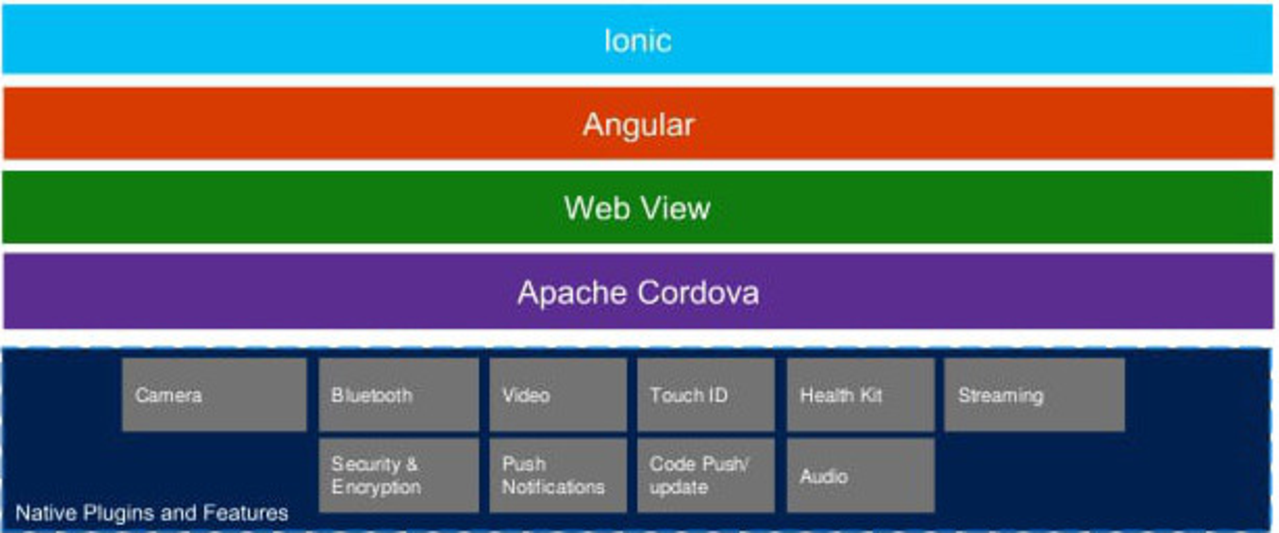
\includegraphics[width=0.2\textwidth]{/img/cordova.pdf}
		\caption{Arquitectura Ionic~\cite{CORDOVAimg}}
		\label{fig:CORDOVAimg}
	\end{center}
\end{figure}



\subsection{React Native}



\subsection{NativeScript}

\section{Aplicaciones de la competencia}
\subsection{Spigit}
\subsection{ideas4all}
\subsection{hypeInnovation}
\subsection{brightIdea}
https://play.google.com/store/apps/details?id=com.brightidea.mobile5
\subsection{exago}

% Local Variables:
%  coding: utf-8
%  mode: latex
%  mode: flyspell
%  ispell-local-dictionary: "castellano8"
% End:
